%%%%%%%%%%%%%%%%%%%%%%%%%%%%%%%%%%%%%%%%%
% Journal Article
% LaTeX Template
% Version 1.3 (9/9/13)
%
% This template has been downloaded from:
% http://www.LaTeXTemplates.com
%
% Original author:
% Frits Wenneker (http://www.howtotex.com)
%
% License:
% CC BY-NC-SA 3.0 (http://creativecommons.org/licenses/by-nc-sa/3.0/)
%
%%%%%%%%%%%%%%%%%%%%%%%%%%%%%%%%%%%%%%%%%

%----------------------------------------------------------------------------------------
%	PACKAGES AND OTHER DOCUMENT CONFIGURATIONS
%----------------------------------------------------------------------------------------

\documentclass[twoside]{article}


\usepackage{graphicx}
\usepackage{lipsum} 

\usepackage[sc]{mathpazo} % Use the Palatino font
\usepackage[T1]{fontenc} % Use 8-bit encoding that has 256 glyphs
%\linespread{1.05} % Line spacing - Palatino needs more space between lines
\usepackage{microtype} % Slightly tweak font spacing for aesthetics

\usepackage[hmarginratio=1:1,top=32mm,columnsep=20pt]{geometry} % Document margins
\usepackage{multicol} % Used for the two-column layout of the document
\usepackage[hang, small,labelfont=bf,up,textfont=it,up]{caption} % Custom captions under/above floats in tables or figures
\usepackage{booktabs} % Horizontal rules in tables
\usepackage{float} % Required for tables and figures in the multi-column environment - they need to be placed in specific locations with the [H] (e.g. \begin{table}[H])
\usepackage{hyperref} % For hyperlinks in the PDF

\usepackage{lettrine} % The lettrine is the first enlarged letter at the beginning of the text
\usepackage{paralist} % Used for the compactitem environment which makes bullet points with less space between them
\usepackage{sectsty}

\usepackage{titlesec} % Allows customization of titles
\titleformat{\section}[block]{\large\scshape}{\thesection.}{1em}{} % Change the look of the section titles
\titleformat{\subsection}[block]{}{\thesubsection.}{1em}{} % Change the look of the section titles


%----------------------------------------------------------------------------------------
%	TITLE SECTION
%----------------------------------------------------------------------------------------

\title{\vspace{-15mm}\fontsize{20pt}{10pt}\selectfont\textbf{NLP report}} % Article title

\author{
\large
\textsc{Ge Gao  gg24984}\\[2mm] % Your name
\normalsize \href{mailto:gegao1118@utexas.edu}{gegao1118@utexas.edu}
\vspace{-5mm}
}
\date{}

%----------------------------------------------------------------------------------------
\begin{document}

\maketitle % Insert title


%----------------------------------------------------------------------------------------
%	ARTICLE CONTENTS
%----------------------------------------------------------------------------------------

\begin{multicols}{2} % Two-column layout throughout the main article text


%========================================================================================
% Problem Statement
\section{Introduction}
Question Classification(QC) is a task that given a question, some classifier will map this question to one of k limited classes, so that a semantic constraint will be put on this question, which will make potential machine translation or automatic answering easier.  


%========================================================================================
\section{Related Work}
\subsection{Question classifiers}
In the ``Learning Question Classifier'' paper(Li and Roth, 2002), in terms of the question classification task, the number of question types(k) could be either six or fifty depending on different classification criteria.  Li and Roth developed a machine learning method to classify questions which is guided by a layered semantic hierarchy of answer types. They made use of a sequence of two simple classifiers to do the classification. The first classifies questions into coarse classes (six in total) and second classifies questions into fine classes(fifty in total). And the second classifier is also dependent on the first one. Here is the structure of the hierarchical classifier by Li and Roth.
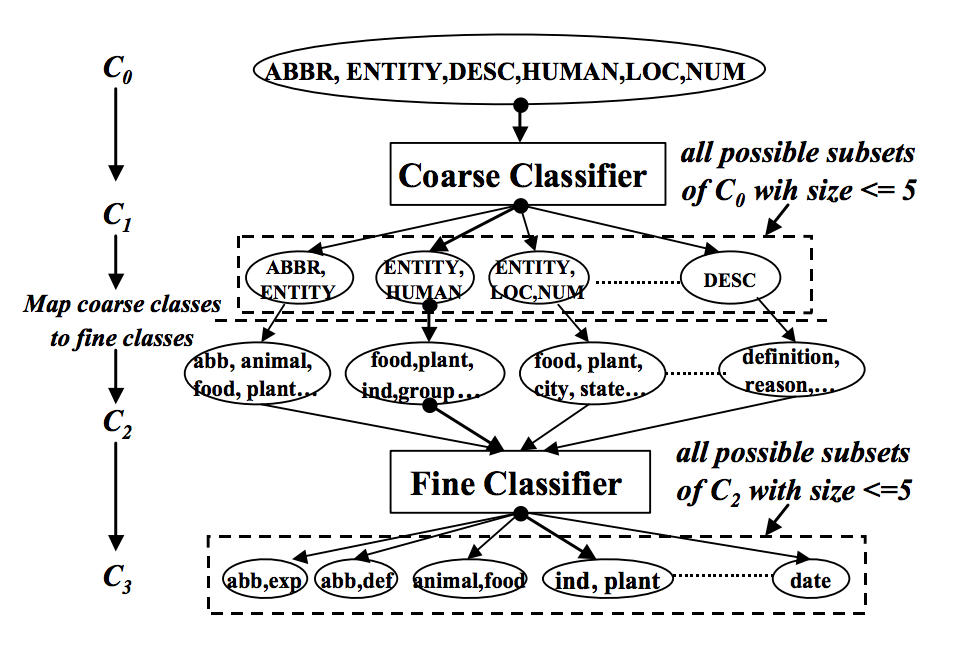
\includegraphics[width=0.5\textwidth]{structure.png}
\begin{center}
Figure1:  The hierarchical classifier 
\end{center}
Figure 1 shows the basic classification process by classifier by Li and Roth. A question will always be processed along a top-down path to be classified. And after the classification process, question type labels will be attached to the question.
\\In Li and Roth's classifier, each question is analyzed as a list of features so that they could be trained and tested for learning.They extracted some primitive features like words, pos tags and chunks (Abney, 1991), named entity as well as some semantically related words. Based these features, they compose and make some more complex features. Also, they make a semantically related word list for most question types. For example, ``far'' is in the semantically related words of ``distance'' so that if there is an occurrence of ``far'', and then the sensor for ``distance'' will be activated and the feature will be extracted.
\\A point that is worth pointing out is that there might be some ambiguity for some specific questions. For example, a question like ``What do bats eat'' could either be classified to belong to food type or animal type, and both them can make much sense. To solve this, Li and Roth allow multiple type labels to be attached to a single question.

\subsection{CNN on sentences classification}
Convolutional neural networks(CNN) model is a deep learning which has achieved many remarkable results in many fields and in the model developed by Yoon Kim(2014), A CNN model was developed for sentence classification which accepts word vectors as input and type labels as output.
\\Convolutional neural networks was originally invented for tasks in computer vision fields and was proved to be also effective in many NLP tasks. In Kim' model, they train one layer of filter on top of word vectors generated by word2vec developed by Google(Mikolov et al 2013). In Kim's model, there are ``static'' and ``nonstatic'' for model variation, where ``static'' means that the vectors are directly from word2vec and for ``nonstatic'', those vectors will also be tuned for each data set.



\section{baseline of Kim's model}
Because Kim's model that is available from his GitHub is for Google news, so we made some modifications based on his code and did the replicating experiment for TREC 10.


\end{multicols}
\end{document}

